% !TeX spellcheck = fr_FR
\documentclass[12pt,a4paper]{report}
\usepackage{style/preambule_college}
\usepackage{style/preambule_personnalisation}
\usepackage{geometry}
\usepackage{amsmath}
\usepackage{tikz}
\usepackage{xcolor}
\usepackage{pgfplots}
\chapterFormat


\begin{document}
	\chapter[Analyse]{Fonction exponentielle et logarithmique}
	\section*{Fonction exponentielle}
	\subsection*{Définition et Graphe}
	Soit $a \in \mathbb{R}^{*}_{+} \backslash \{1\}$. La fonction exponentielle de base $a$, notée $\exp_{a}$, est définie par: \[ \exp_{a}: \mathbb{R} \rightarrow \mathbb{R}^{*}_{*}\] \[x \rightarrow y=a^{x} \]
	
	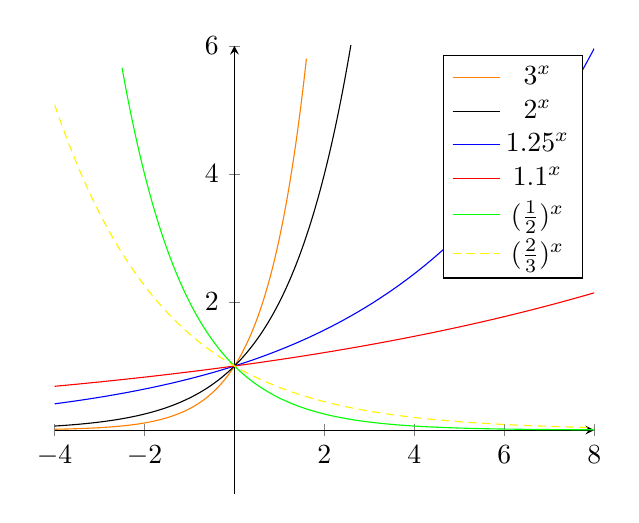
\begin{tikzpicture}
	\begin{axis}[
	xscale=1,yscale=1,
	xmin=-4, xmax=8,
	ymin=-1, ymax=6,
	samples=1000,
	axis lines=center,
	]
	\addplot+[domain=-4:1.6,mark=none,orange] {3^x};
	\addlegendentry{$3^x$}
	\addplot+[domain=-4:4.5,mark=none,black] {2^x};
	\addlegendentry{$2^x$} 
	\addplot+[domain=-4:8,mark=none,blue] {1.25^x};
	\addlegendentry{$1.25^x$}
	\addplot+[domain=-4:8,mark=none,red] {1.1^x};
	\addlegendentry{$1.1^x$}
	\addplot+[domain=-2.5:8,mark=none,green] {0.5^x};
	\addlegendentry{$(\frac{1}{2})^x$}
	\addplot+[domain=-4:8,mark=none,yellow] {0.666^x};
	\addlegendentry{$(\frac{2}{3})^x$}
	\end{axis}
	\end{tikzpicture}
	\subsection*{Propriétés}
	\begin{enumerate}
		\item $\exp_{a}(0)=a^0=1$
		\item $\exp_{a}(1)=a^1=a$
		\item $a^{x+y}=a^x\cdot a^y$
		\item $a^{x-y}=\frac{a^x}{a^y}$
		\item $(a^x)^m=a^{mx}$
		\item $\forall x \in \mathbb{R}^{*}_{+}$ :
		$\begin{cases}
			a>1 &\Rightarrow a^x>1 \\
			0<a<1 &\Rightarrow 0<a^x<1
		\end{cases}$
	\end{enumerate}
	\subsection*{Croissance}
	La fonction exponentielle de base $a$ est:
	\begin{itemize}
		\item strictement croissante si $a>1$: ($a>1 et x<y) \Rightarrow a^x<a'y$
		\item strictement décroissante si $0<a<1$: ($0<a<1$ et $x<y$) $\Rightarrow a^x>a^y$
	\end{itemize}
	\subsection*{Limite}
	\[ a>1, \hspace{1cm} \lim\limits_{x \Rightarrow +\infty} a^x=+\infty \hspace{1cm} \lim\limits_{x \Rightarrow -\infty} a^x=0 \]
	\[ 0<a<1, \hspace{1cm} \lim\limits_{x \Rightarrow +\infty} a^x=0 \hspace{1cm} \lim\limits_{x \Rightarrow -\infty} a^x=+\infty \]
	\subsection*{Autre}
	La fonction $\exp_{a}$ est définie et continue sur $\mathbb{R}$ et c'est une bijection de $\mathbb{R}$ vers $\mathbb{R}^{*}_{+}$
	\section*{Fonction logarithme}
	A la fonction $\exp_{a}$ c-à-d $a^x=y$ correspond sa réciproque appelée $\log_{a}$ c-à-d $x= \log_{a}(y)$.
	\subsection{Définition et graphe}
	La fonction $\log_{a}$, (pour $a \in \mathbb{R}_{+}^{*} \backslash\{1\}$) est définie par \[\mathbb{R}_{+}^{*} \rightarrow \mathbb{R}\]
	\[x\rightarrow y=\log_{a}(x)\]
	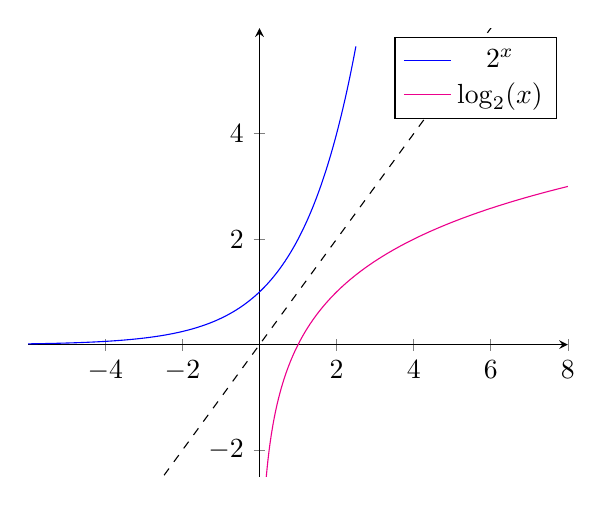
\begin{tikzpicture}
	\begin{axis}[
		xscale=1,yscale=1,
		xmin=-6, xmax=8,xtick={-4,-2,0,2,4,6,8},
		ymin=-2.5, ymax=6,ytick={-2,0,2,4},
		samples=1000,
		axis lines=center,
		]
		\addplot+[domain=-6:2.5,mark=none,blue] {2^x};
		\addlegendentry{$2^x$}
		\addplot+[domain=0:9,mark=none,magenta] {ln(x)/ln(2)};
		\addlegendentry{$\log_{2}(x)$}
		\addplot+[domain=-4:8,mark=none,black,dashed] {x};
	\end{axis}
	\end{tikzpicture}
	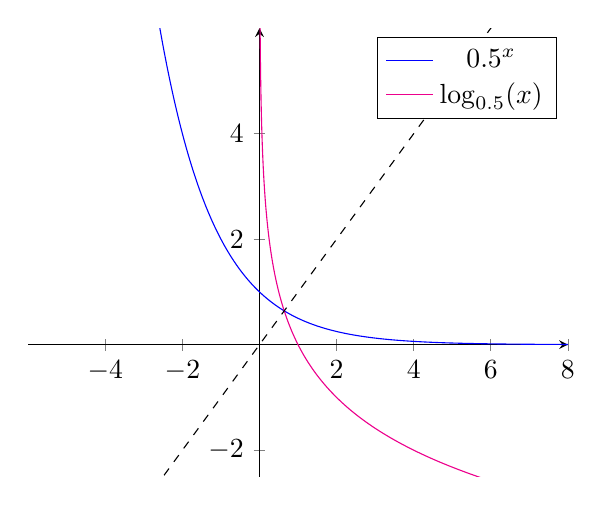
\begin{tikzpicture}
	\begin{axis}[
		xscale=1,yscale=1,
		xmin=-6, xmax=8,xtick={-4,-2,0,2,4,6,8},
		ymin=-2.5, ymax=6,ytick={-2,0,2,4},
		samples=1000,
		axis lines=center,
		]
		\addplot+[domain=-3:10,mark=none,blue] {0.5^x};
		\addlegendentry{$0.5^x$}
		\addplot+[domain=0:8,mark=none,magenta] {ln(x)/ln(0.5)};
		\addlegendentry{$\log_{0.5}(x)$}
		\addplot+[domain=-4:8,mark=none,black,dashed] {x};
	\end{axis}
	\end{tikzpicture}
	\subsection*{Propriétés}
	Soit $a \in \mathbb{R}_{+}^{*}\backslash \{1\}$
	\begin{enumerate}
		\item $\log_{a}(1)=0$
		\item $\log_{a}(a)=1$
		\item $\log_{a}(x\cdot y)=\log_{a}(x)+\log_{a}(y) $
		\item $\log_{a}(\frac{x}{y})=\log_{a}(x)-\log_{a}(y)$
	\end{enumerate}
	\subsection*{Croissance}
	La fonction $\log_{a}$ est une bijection continue de $\mathbb{R}_{+}^{*}$ vers $\mathbb{R}$.
	
	Si $a>1$, $\log_{a}$ est strictement croissante.
	
	Si $0<a<1$, $\log_{a}$ est strictement décroissante.
	\subsection*{Limite}
	Soit $a \in ]1;+\infty[$,\hspace{0.5cm} $\lim\limits_{x \Rightarrow 0_{+}} a^x=-\infty$ \hspace{0.5cm} et \hspace{0.5cm} $\lim\limits_{x \Rightarrow +\infty} a^x=+\infty$
	\subsection*{Autre}
	\begin{enumerate}
		\item $\log_{10}(x)=\log(x)$ est appelé logarithme décimal
		\item Soit $n \in \mathbb{Z}$, $\forall x \in \mathbb{R}_{+}^{*}$ tel que $10^n \leqslant x < 10^{n+1}$, $E(log(x))=n$
		\begin{itemize}
			\item Si $x \in \mathbb{N}^{*}$, alors $x$ s'écrit avec $E(\log(x))+1$ chiffres
			\item Si $x \in ]0;1[$, alors l'écriture décimale de $x$ commence par -$E(\log(x))$ zéros, en comptant celui situé avant la virgule.
		\end{itemize}
	\end{enumerate}
	\section*{Le nombre $e$}
	
	Soit $f(x) = a^x$. Cherchons une base notée $e$, telle que $f'(0)=1$. Par définition de la dérivée d'une fonction: 
	\begin{align*}
		f'(0) & = \lim\limits_{h \rightarrow 0} \frac{a^h-1}{h} \quad \text{qui est une forme indéterminée} \\
		\text{et} \quad f'(x) & = \lim\limits_{h\rightarrow 0}\frac{a^{x+h}-a^x}{h}= \lim\limits_{h\rightarrow 0} \frac{a^xa^h-a^x}{h} \\
		&= a^x \lim\limits_{h \rightarrow 0} \frac{a^h-1}{h} = a^xf'(0)
	\end{align*}
	en remplaçant $a$ par $e$, on a : $(e^x)' =f'(x)=(e^x)$.
	
	\medskip
	On cherche donc une base notée $e$, telle que \hspace{0.5cm} $\lim\limits_{h \rightarrow 0} \frac{e^h-1}{h}=1$
	
	\medskip
	Ce qui nous donne pour $h$ proche de 0: \[ e^h-1\approx h \Leftrightarrow e^h \approx 1+h \Leftrightarrow e \approx (1+h)^{\frac{1}{h}} \]
	
	\medskip
	En posant $n=\frac{1}{h}$, $h \rightarrow 0 \Leftrightarrow n \rightarrow \pm \infty$, on obtient: \hspace{0.4cm} $e \approx \left(1+\dfrac{1}{n}\right)^n$
	
	Un résultat généralisé existe: \[\lim\limits_{x \rightarrow \pm \infty} \left(1+\dfrac{a}{x}\right)^x=e^a \]
	
	\medskip
	Le $\log_{e}(x) = ln(x)$ appelé le logarithme naturel.
	\section*{Dérivée des fonctions $\exp_{a}$ et $\log_{a}$ }
	\subsection*{Exp}
	\begin{align*}
	\text{La fonction est dérivable sur} \hspace{0.1cm} \mathbb{R} \\
	(e^x)' = e^x \\
	(a^x)' = a^x\ln(a) \\
	(e^f)' = e^f\cdot f'
	\end{align*}
	\subsection*{Log}
	\begin{align*}
	\text{La fonction est dérivable sur} \hspace{0.1cm} \mathbb{R}^{*}_{+} \\
	(\log_{a}(x))' &= \frac{1}{\ln(a)}\cdot\frac{1}{x} \\
	(\ln(x))' &= \frac{1}{x}
	\end{align*}
\end{document}